% Your independent working draft. Start writing below \maketitle.
% Target: Physical Review E, Network Science for Understanding AI.
% Change reprint to preprint for a single-column editing view.
\documentclass[aps,pre,reprint,superscriptaddress,longbibliography]{revtex4-2}
\usepackage{amsmath,amssymb,amsthm}
\usepackage{bm}
\usepackage{graphicx}
\usepackage{booktabs}
\usepackage[hidelinks]{hyperref}

\newcommand{\R}{\mathbb{R}}
\newcommand{\ones}{\mathbf{1}}
\newcommand{\norm}[1]{\left\lVert #1 \right\rVert}
\newcommand{\abs}[1]{\left\lvert #1 \right\rvert}
\DeclareMathOperator{\vol}{vol}
\DeclareMathOperator{\diag}{diag}
\DeclareMathOperator{\rank}{rank}
\DeclareMathOperator{\col}{col}

\newtheorem{theorem}{Theorem}
\newtheorem{lemma}[theorem]{Lemma}
\newtheorem{corollary}[theorem]{Corollary}
\theoremstyle{remark}
\newtheorem{remark}[theorem]{Remark}


\begin{document}

\title{Working title}
% Copied from paper/current/main.tex on 2026-10-29; edit as needed.
\author{Govind Gandhi}
\affiliation{School of Data Science, University of Virginia, Charlottesville, Virginia 22904, USA}
\author{Sadamori Kojaku}
\affiliation{School of Systems Science and Industrial Engineering, Binghamton University, Binghamton, New York 13902, USA}
\author{Yong-Yeol Ahn}
\email{yyahn@virginia.edu}
\affiliation{School of Data Science, University of Virginia, Charlottesville, Virginia 22904, USA}


\begin{abstract}
For skip gram embeddings, where a latent property like degree or community membership ends up in the geometry is important. 
We identify the factors by embeddings DCSBM networks since it lets us clamp down and establish the factors unlike text. 
They give us "ground truth" and exact targets and data whose latent variables (degree and community) we can control. 
The findings then help explain the norm-frequency behavior of word embeddings (as well as an existing puzzle in network science lit).

\end{abstract}

\maketitle


\section{Introduction}
\label{sec:introduction}
% Should we introduce networks and then embeddings, and then justify why we are having one representation move to another? 

% What is network geometry and embeddings

Network Geometry is an approach that abstracts the complex system from nodes and edges of a network into a geometric space. There are many algorithms that embed networks successfully into a latent space. %cite node2vec, a higher order version of embedding, Boguna and Kriukov and Serrano's hyperbolioc method of embedding,network geometry paper,  spectral embedding, etc.
Embeddings offer richer representation and can easily integrate information of nodes/edges/system as we get them. 
Scalable ML tools exist to handle them and for tasks like node/link prediction, classification, clustering, data compression~\cite{hamilton2017representation}.
However, these come at the cost of being less interpretable. 
%We don't want to give up the predictive performance, efficiency and scalability; can we say more about interpretability?


Multiple embedding algorithms exist to assign a vector to each node. 
The network doesn't tell us what the norm of a vector or the angle between two vectors should be. 
We must choose what the vectors are meant to represent, and in effect which algorithms do the conversion. 
We could ask vectors to represent the network's raw connection strengths, connections after correcting for how well connected their endpoints are, how frequently two nodes appear together in random walks, how much more often they appear together than expected under a null model, or all of them at the same time. 
The embedding algorithms that convert the network into matrices are constructed to represent the required changes but as advances in machine learning go, the ability of being able to extract many such useful information from the embeddings and use them to tackle many downstream problems have raced ahead of our understanding of what the algorithm is doing to the network information while it's converting the network into a matrix (a bunch of vectors).

One aspect of interpretability is where a known latent property ends up in the geometry (in norms, in directions, or nowhere). Hyperbolic embeddings explicitly construct norms and angles to have degree and community information <cite BOguna serrano et al work>.
We focus on random-walk-based embedding methods such as Node2Vec, which consistently outperform other algorithms on tasks we care about, including classification, community detection, and link prediction~\cite{kojaku2024network, dehghan2022evaluating}.
Random-walk-based methods sample paths through a network and train a predictive model on the resulting node sequences~\cite{perozzi2014deepwalk,grover2016node2vec}.
Many applications, like community detection, use vector directions through cosine similarity. The vector norm is nevertheless a second observable that can encode network properties as well, such as node frequency, context, and information from training dynamics.
Its interpretation matters whenever embeddings enter a dot product \cite{steck2024cosine}.
What factors contribute to where a known property of the network/text data ends up in the geometry of skip gram based embeddings? 

% Figure generated by scripts/step0/figure_paper.py (data: results/step0/runs, Figshare 13072790, KDD Cup 2003 hep-th, BlogCatalog).
\begin{figure*}[t]
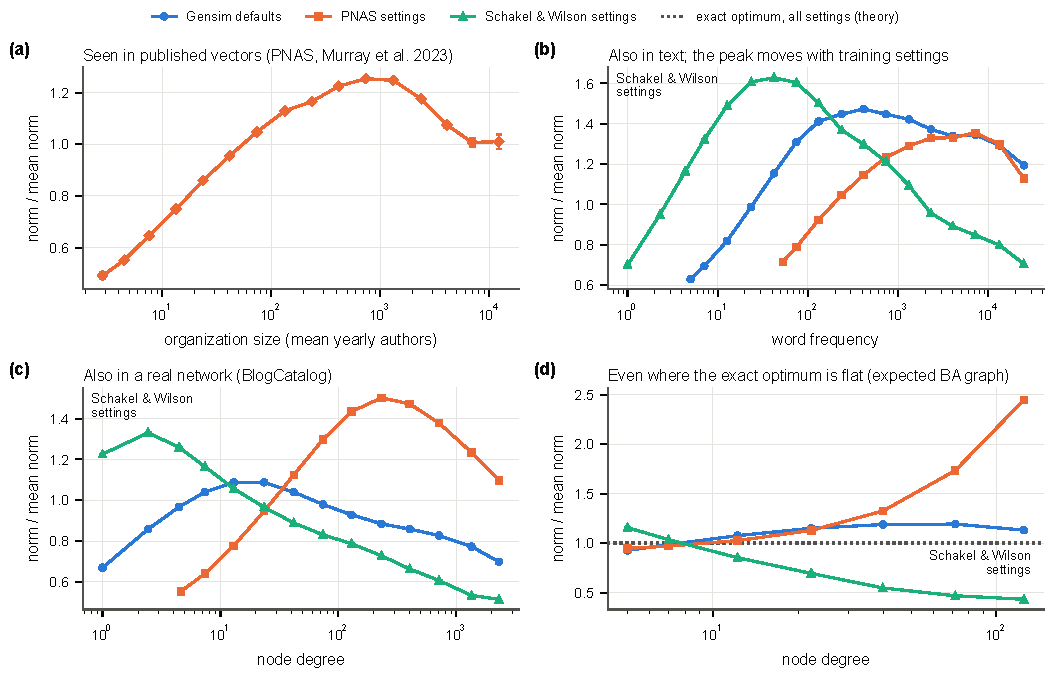
\includegraphics[width=\textwidth]{figures/fig1_problem.pdf}
\caption{Skip-gram vector norms vary strongly with frequency---rising and then falling in published vectors, in text and in a real network---and vary even on a synthetic graph where the exact optimum of the objective has no frequency dependence, differently for each training setting.
Each curve is the raw norm of the center vector divided by its mean over the vocabulary, averaged in log-spaced bins (four per decade) and plotted at the mean logarithm of the binned quantity; error bars are s.e.\ over five seeds and are mostly smaller than the markers; bins with fewer than ten tokens in any seed are omitted. Colors denote training settings and markers distinguish series.
(a) Organization vectors published by Murray \textit{et al.}~\cite{murray2023unsupervised} (diamonds; trained with the PNAS settings), against organization size (mean yearly number of authors); error bars are s.e.\ over organizations.
(b) Embeddings of 29\,555 hep-th titles and abstracts, the corpus of Schakel and Wilson~\cite{schakel2015measuring}; their published settings are the third series in (b)--(d).
(c) Embeddings of random walks on the BlogCatalog social network~\cite{tang2009relational} (10\,312 nodes, 333\,983 edges), a standard benchmark for random-walk embeddings~\cite{perozzi2014deepwalk,grover2016node2vec}: ten walks per node of 80 steps, started in proportion to degree, each step to a uniformly chosen neighbor.
(d) Walks on the expected graph, at fixed degrees, of a Barab\'asi--Albert graph~\cite{barabasi1999emergence} ($N=10^4$, $m=5$; one realization per seed), which links every pair of nodes with weight proportional to the product of their degrees, so that every token is an independent draw in proportion to degree; walk number and length as in (c). The dotted line is the exact optimum of the expected loss under all three settings: every center vector is identical, in any factorization gauge, so the normalized norm is 1 (in the balanced gauge the common norm is 1.31 under Gensim defaults, 1.27 under PNAS settings and 1.28 under Schakel \& Wilson settings).
Gensim defaults: 100 dimensions, window 5, negative-sampling exponent 0.75, subsampling $10^{-3}$, 5 epochs, minimum count 5.
PNAS settings~\cite{murray2023unsupervised}: 300 dimensions, window 1, exponent 1, 5 epochs, minimum count 50; subsampling off (not reported).
Schakel \& Wilson settings~\cite{schakel2015measuring}: 100 dimensions, window 10, subsampling $10^{-4}$, 20 epochs, minimum count 1.
Under PNAS settings the minimum count removes 12\% of BlogCatalog nodes (those of degree three or less and about half of those of degree four); it removes no nodes in (d) and almost none in (c) under the other settings.}
\label{fig:problem}
\end{figure*}

Vector norms in skip-gram embeddings vary strongly with frequency.
In the organization vectors of Murray \textit{et al.}~\cite{murray2023unsupervised}, the norm rises with organization size and then falls (Fig.~\ref{fig:problem}(a)); word vectors show the same rise and fall with word frequency~\cite{schakel2015measuring} (Fig.~\ref{fig:problem}(b)), and so do node vectors on a standard network benchmark (Fig.~\ref{fig:problem}(c)).
Where the peak sits depends on the training settings, not only on the data (Fig.~\ref{fig:problem}(b),(c)).
A natural reading is that a norm measures how informative a word's or node's contexts are~\cite{schakel2015measuring,oyama2022norm}, and norm--frequency questions arise for token embeddings in language models as well.
We would like to know where the curve comes from.
In text, these questions are harder to settle because you don't know the ground truth, these is no true frequency and true topic for a word to recover. 
Networks can give us that sandbox. 
A DCSBM for instance, lets us control degree and community exactly. 
SGNS on random walks has a known closed form target \cite{qiu2018network}.
So unlike in text, we can ask precisely in networks what information survives the conversion from structure to geometry, and where does it end up—norms,angles or neither?
Networks can supply controlled ground truth and exact theory for interpretability questions that are otherwise untestable.

As a first use of this sandbox, take the expected graph of a Barab\'asi--Albert network~\cite{barabasi1999emergence}, which links every pair of nodes with weight proportional to the product of their degrees, so that every node sees the same contexts.
For this graph the closed-form target of Qiu \textit{et al.}~\cite{qiu2018network} is a constant matrix, $M_{ij} = -\log b$ for $b$ negative samples, at any window size.
Gensim's departures from the setting of that closed form (subsampling, the negative-sampling exponent, and skipping negative samples that equal the true context) change the optimal score only through the context node, so the optimum stays rank one with identical rows: every node has the same center vector, at any embedding dimension and under every training setting.
% TODO: write up this derivation (scripts/step0/theory.py docstring; check of Qiu's closed form on the expected graph) in Sec. II or an appendix.
Trained embeddings nevertheless depend on degree, differently for each setting (Fig.~\ref{fig:problem}(d)).
On this graph the norm--degree curve is therefore produced by training, not by the objective.
That conclusion does not yet extend to real networks.
On a sampled graph the target itself contains degree: at window size one, the target of Qiu \textit{et al.} on an edge is $M_{ij} = \log[\vol(G)/b] - \log d_i - \log d_j$~\cite{qiu2018network}, and $-\infty$ off the edges.
There the curve can come from the objective, from training, or from both, and a norm cannot be read as information about a node until we can tell them apart.
% TODO (needed to extend the claim to sampled graphs): compute the rank-d optimum X* of the exact loss on the sampled graph and compare its balanced norms with the trained ones, as Fig. 1(d) does for the expected graph. At window 1 every non-edge has optimal score -infinity, so use a window at least the graph's diameter (every pair co-occurs) or the weighted low-rank optimum (endpoint step of the Plan below).

% End of general introduction






\subsection{Details}% Intro to what we do

Deepwalk, LINE and other skip-gram based network embeddings are very useful but they were treated as "black boxes".
\cite{levy2014neural} showed that SGNS algorithm implicitly factorizes a specific word-context matrix (word2vec). 
\cite{qiu2018network} extends that logic to graphs.

They show that these SGNS methods - LINE, Deepwalk are more than heuristics, they are principled closed-form approximations involving the adjacency and degree matrices of the graph.
% LINE captures 2nd order proximity.
% Deepwalk uses random walks to capture higher order proximity within a window size of T.
% Node2vec introduces two parameters to bias the random walks towards either DFS or BFS.
% Another complication is that unlike DeepWalk's first order RW it uses second order RW.
The derivation confirms that node2vec also performs an implicit matrix factorization, but the target matrix is significantly more complex, involving a higher order transition probability tensor. 
%While the complexity of second order RWs makes the computation difficult, the derivation confirms that node2vec also follows the same principle as its predecessors. 

Our task of interpreting how information flows from network to the embeddings, is now to identify how information from the degree and adjecency matrices transform into the matrix factorizations. All of science is either linear algebra or titration after all.
For instance, how does the node's degree or community membership information exist in the matrix factorization? 
That is, in $M \approx W. C^T $, how does degree information exist in W? The norms, angles, a mixture of both?
This particular example is noteworthy because we see node embeddings have norms that vary with degree~\cite{murray2023unsupervised}, and we would like to know where does that come from? 


%Part 1
We show that the theory says the answer depends on the embedding operator. 
Using DCSBM, we derive the exact geometry of several things.
For spectral embeddings of the normalized adjacency matrix and for the raw probabiooities that two nodes co-occur on a random walk, the geometry separates exactly: within a community, degree sets the vector's length and community alone sets its direction. 
For the target that SGNS optimizes, the separation fails. 
With the standard unigram negative sampling distribution, degree cancels out entirely on the expected graph.
With other engative sampling exponents, degree reappears only on the context side, as necessarily affecting the direction, rather than as length. 
This tells us that on the expected graph any norm--degree pattern must come from the training process, not from the objective (Fig.~\ref{fig:problem}(d)).
The norm--degree patterns we see in practice <find and cite more such instance> are on sampled graphs, whose edges put degree back into the target, so there the same conclusion still needs the optimum for each graph.

%Part 2
%Being able to tackle such questions have an implementational hurdle.
Let's understand why that's the case. 
We only know that there exists a matrix M that can be written as W.C (Transpose) - a matrix product of the centre and context vectors of nodes in the network.
However, M is not built, its the emergent approximation as an objective function nears an optimum.
For SGNS, random walks are obtained from the network, and the objective rewards high scores on real pairs, and low scores on negative samples.
Ref. \cite{qiu2018network} tells us the closed form of M in this case for a network.

However, knowing the matrix factorization product exactly doesn't pin down the matrices in the product - W and C.
The two matrix products W and C can be stretched and sheared in a way to give the same product i.e. there's a gauge freedom (W. R. R-1 . CT = W' . C'T = M | W' = WR, C' = C(R-1)).

Does this gauge fixing determine which network information goes to the embeddings that we use (W) and the context matrix that we discard (C).
Furthermore, how does it decide which information in M is expressed geometrically inside W?

\footnote{<TODO: existing research seems to indicate that gauge freedom can be removed by normalizing* https://www.tahabouhsine.com/relevatio/blogs/cosine/main.pdf , which was a response to \cite{steck2024cosine}, which raises correctly that cosine sims of embeddings trained on dot similarity objective can yield arbitrary results and meaningless similarities. >}

Node2vec's recipe can be implemented in many ways, and sometimes those implementation details can constrain and sometime implicitly remove this freedom entirely. 
note that the implementations still can capture their objective, which could be interpreted as community structure, because that comes from node co-occurence information from the random walks. 
They can disagree mainly in how much degree information they keep and where they put it. 
Which is what we are interested in.

Interpreting a norm requires understanding the embedding operator, the negative sampling distribution, the factorization gauge, the training exposure, etc (inexhaustive list)

Update this: Right now the paper experimentally isolates exposure and context to see how that affects the curve we observe. Shows that we can bend the U shape using these factors. But that doesn't confirm that our theory is right. Nor does it get into the implementation theory of how these factors shape the norm info. 



Can we divide information into the matrices and how they are expressed geometrically in a more controllable and interpretable way?


Can this extend to specifying which information goes to which parts of a vector for instance to the norms, angles, etc?




\section{Model and methods}
\label{sec:methods}

*\subsection{The Plan} %Will delete later, only for placeholder and reference
\begin{itemize}
    \item To understand generally how network info gets into geometry of embedding, we need to look at M given proof that SGNS factorizes almost exactly. You can go bottom up, how does degree show up in embedding? You can also ask what network info resides in the norms?
    
    \item What determines which info goes how to W in $W . C^T = M$?
    1. Need to know M and 2. which factorization it undergoes to get W. 
    Gensim is the default method, so we focus on its method and default parameters.
    Under gradient flow, imbalance between initial W and C is preserved throughout training, and gensim supposedly preserves balanced factorization.
    This factorization is unique up to a rotation, and rotations preserve norms and angles (given that's our interest right now).
    We want to check whether route 2 is closed, that is whether whatever M training reaches, it always splits it the same way (balanced). 
    If so, two models that reach the same M have the same norms and angles, however they were trained. Two models with different norms must have reached different M.
    We check this for all the runs. If the gradient flow agrees and the W and C are close to balanced factorization (that's a heuristic), and more importantly SVD of M yields balanced factorized matrices then W's geometry is a function of the reached product alone. 
    This also implies cosine similarities are not arbitrary (response to steck et al)
    (if route 2 is closed, great, just study the M directly, we can compare the reached M with the optimal M to fully explain the norms)
    (If route 2 is open, exposure could also change norms through the split, then we need a model of the gauge as well as of M :'/)

    \item So now if the reached M in training is different from its ideal version from the theory, then only reason is training stopped prematurely.
    How do we reliably find the endpoint? We can use Qiu et al's M provided we align gensim with its 4 assumptions.
    We can align 3 of them easily - window weights, negative sampling exponent, subsampling, finite walks, 
    Ideal trained matrix X* can only be a weighted low rank approximation of M.
    Theory departs here, we have to numerically do the minimization from M to get an X*.
    Train gensim far longer than usual, and empirical check its WCt and its balanced norms approach X*. 
    If they don't, go back and fix the gensim alignment
    
    \item How do we check how degree is encoded in the endpoint?
    We know W is the balanced factor of product, so we can SVD X* as well into a balanced factor W. 
    Plot Degree-norm curve of 4 different things:
    (z. On DCSBM graphs, also compute a. on the expected graph, difference from A shows how much degree comes from graph being a finite sample, this is the only link the existing theorems)
    a. Qiu's M with settings matched to gensim (M has to be finite, run at large enough window for every pair to co-occur)
    b. X* rank d optimum of exact loss 
    c. Gensim's WCt after normal training
    A to B answers effect of limited dimension. B to C is effect of training stopping early.
    See where U shape shows up.
    %For alpha=1, degree cancels out from the paper, makes it easier to see that.

    \item Changes based on previous results. But assuming earlier reasoning, U shape shows up at training.
    We explain the gap between the endpoint and trained model.
    Split norm into ideal and trained, see if you can write trained norm as a function of ideal times factors.
    Best candidate is 

\end{itemize}

Training parameters and implementation details of different algorithms of the same embedding method can still affect the W matrix because they can get to the product matrix and the embedding vectors in different ways.
Gensim and Pytorch are two popular implementations of Node2vec. 
However, Pytorch sets W=C so that the model fits W WT ~ M, this has no gauge freedom to fix. 
Some of M can't be representated this way, since this product can never have negative eigenvalues this way. For most graphs this matters little, but it matters for (near) bipartite graphs.

Gensim, has a variable, nsexponent that determines how frequently nodes are sampled for negative samples. 
Setting it to 1 means nodes are sampled for negative context exactly proportional to their structural frequency in the random walks. 
Whereas 0 sets all nodes to be sampled equally, disregarding their frequency in walks. 
Gensim defaults to 0.75 middle ground as it softens the dominance of hubs (while still maintaining its behaviour) while elevating lower frequency nodes 



Even after all this, fixing training hyperparameters give a consistent experimental setup, but each graph can still produce a distribution of node2vec embeddings across runs~\cite{hacker2022surprising}. 
So we would need to distinguish variation caused by network structure from variation caused by training to confirm our theoretical findings. 


\section{Results}
\label{sec:results}


\section{Discussion}
\label{sec:discussion}


% Add these when there is content for them:
% \begin{acknowledgments}
% \end{acknowledgments}
%
% \section*{Data availability}
%
% \appendix
% \section{Additional derivations}
% \label{app:derivations}

% Show the entire library while drafting. Remove this line before submission
% so that only works actually cited in your text appear in the references.
\nocite{*}
% REVTeX selects apsrev4-2 automatically and passes longbibliography controls.
\bibliography{references}

\end{document}
